%форматирование размера документа
\documentclass[11pt, a4paper]{article}

\usepackage{geometry}
% total - determines printable width, height
\geometry{ 
	a4paper, total={160mm,267mm}
}

%----text,fonts------------------------------------------------------------------------------------
\usepackage{mmap}
\usepackage[T2A]{fontenc}
\usepackage[utf8]{inputenc}
\usepackage[english, russian]{babel}
\usepackage{setspace}
\setstretch{0,9}
\usepackage{fancyvrb}

%----math,graphics---------------------------------------------------------------------------------
\usepackage{amsmath,amsfonts,amssymb}
\usepackage{amsthm}
\usepackage{listings}

\usepackage{tikz}
\usetikzlibrary{calc}
\usepackage{pgfplots}
\pgfplotsset{
	compat=1.17
}

\usepackage{graphicx}
\graphicspath{{image/}}

\usepackage{wrapfig}
\usepackage{tabularx}

% relative importing
\usepackage{import}


\begin{document}

\import{.}{titular.tex}
\newpage

\section{Описание метода. Расчетные формулы}

Метод Адамса позволяет решать дифференциальные уравнения первого порядка. Формулы выводятся из
многочлена Лагранжа. Для вычисления значения данной функции необходимо знание 4 предыдущих значений
функции. Данные значения могут быть найдены с помощью другого метода, одношагового, которым
требуется только условие Коши, например, метода Рунге-Кутты 4-ого порядка.

\medskip\noindent
Формулы для метода Рунге-Кутты 4-ого порядка:
\begin{align*}
  y_{i + 1} &= y_i + \Delta y_i, & i = 1, \dots, n \\
  \Delta y_i &= \frac{h}{6} (K_1 + 2 K_2 + 2 K_3 + K_4) \\
  K_1 &= f(x_i, y_i) \\
  K_2 &= f(x_i + \frac{h}{2}, y_i + \frac{h}{2}K_1) \\
  K_3 &= f(x_i + \frac{h}{2}, y_i + \frac{h}{2}K_2) \\
  K_4 &= f(x_i + h, y_i + h \cdot K_3)
\end{align*}

\medskip \noindent
Формулы для метода Адамса:
\begin{align*}
  \widetilde{y}_{i + 1} &= y_i + \frac{h}{24}(-9 f(x_{i - 3}, y_{i - 3}) + 37 f(x_{i - 2}, y_{i -
  2}) - 59 f(x_{i - 1}, y_{i - 1}) + 55 f(x_{i}, y_i)) \\
  x_{i - 1} &= x_i + \frac{h}{24} (f(x_{i - 2}, y_{i - 2}) - 5 f(x_{i - 1}, y_{i - 1}) + 19 f(x_{i},
  y_{i} + 9 f(x_{i + 1}, \widetilde{y}_{i + 1}))
\end{align*}

\noindent
Вторая формула уточняет первую, является корректирующей.

\section{Блок схема численного метода.}


\begin{figure}[h]
  \centering
  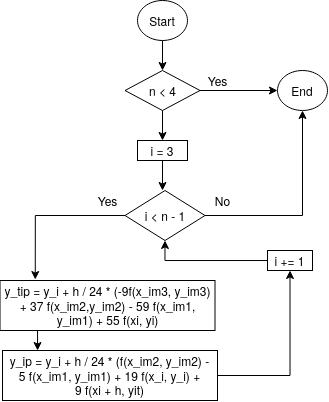
\includegraphics[width=0.5\linewidth]{block.png}
  \label{fig:result-png}
\end{figure}


\newpage
\section{Листинг реализованного численного метода.}

\begin{Verbatim}[fontsize=\small]
def runge_kutta_solve(x0, y0, func, h, n):
    points = []
    x_cur = x0
    y_cur = y0
    points.append({"x": x_cur, "y": y_cur})
    for _ in range(1, n):
        ki1 = func(x_cur, y_cur)
        ki2 = func(x_cur + h / 2, y_cur + h / 2 * ki1)
        ki3 = func(x_cur + h / 2, y_cur + h / 2 * ki2)
        ki4 = func(x_cur + h, y_cur + h * ki3)
        dyi = h / 6 * (ki1 + 2 * ki2 + 2 * ki3 + ki4)
        x_cur += h
        y_cur += dyi
        points.append({"x": x_cur, "y": y_cur})
    return points

def adams_solve(points, func, h, n):
    if (len(points) < 4):
        raise ProjectException("len(points) < 4")
    new_points = points[0:4].copy()
    for i in range(3, n - 1):
        xim3, xim2, xim1, xi = [p["x"] for p in new_points[(i - 3):(i + 1)]]
        yim3, yim2, yim1, yi = [p["y"] for p in new_points[(i - 3):(i + 1)]]
        yit = yi + h / 24 * (-9 * func(xim3, yim3) + 37 * func(xim2, yim2) -
                              59 * func(xim1, yim1) + 55 * func(xi, yi))
        yip1 = yi + h / 24 * (func(xim2, yim2) - 5 * func(xim1, yim1) + 19 * func(xi, yi) +
                              9 * func(xi + h, yit))
        new_points.append({"x": xi + h, "y": yip1})
    return new_points
\end{Verbatim}

\section{Примеры и результаты работы программы на разных данных.}

\noindentВвод данный через ifile:

\begin{Verbatim}[fontsize=\small]
{
  "equation": "\\sin(x) + y",
  "real_eq": "1 / 2 * (5 * \\e^x - \\sinx - \\cosx)",
  "dependant": "y",
  "step": 0.1,
  "count": 20,
  "initial": {
    "x": 0,
    "y" : 2
  }
}
\end{Verbatim}


\begin{figure}[h]
  \centering
  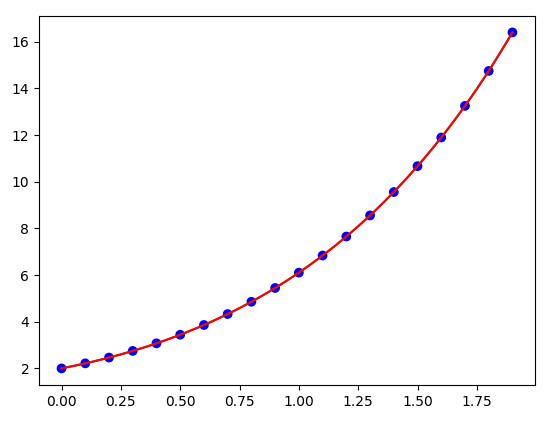
\includegraphics[width=0.5\textwidth]{result.png}
  \label{fig:result-png}
\end{figure}


\section{Вывод.}

В данной лабораторной работе для вычисления первых 4 точек используется метод Рунге-Кутты, его
значение уточняется 4 раза, что выше метода Эйлера, btw метод Эйлера - частный случай метода
Рунге-Кутты. Оба этих метода являются одношаговыми, то есть вычисляются базируясь только на
предыдущем значении.

\medskip\noindent
В отличии от одношаговых методов, многошаговые методы используют значения не только основываясь на
одном предыдущем значении, например, метод Адамаса использует 4 предыдущие точки. Метод Адамаса использует под
капотом полином Лагранжа, а метод Милна - полином Ньютона. То есть по сути эти методы об одном и том
же, но используют разные формулы под интегралом.

\smallskip \noindent
Сам интеграл: \[
y(x_{i + 1}) = x_i + \int_{x_i}^{x_i + 1} f(x, y(x)) dx
.\] 

\medskip\noindent
Недостаток многошаговых методов: тяжело менять шаг в процессе выполнения программы, при смене шага
и при старте требует использования одношаговых методов, а порядок аппроксимации зависит от первых
этих точек. Одного их преимущества над одношаговыми: проще вычислять погрешность, а также порядок
погрешности не уменьшается при увеличении количества точек.
\end{document}

